\documentclass[12pt, letterpaper]{article}
\usepackage[spanish]{babel}
\usepackage[utf8]{inputenc}
\usepackage{graphicx}
\usepackage{amssymb}
\graphicspath{{./imagenes/}}
\usepackage{xcolor}

%Paquetes para símbolos y entornos matematicos. En este documento se usa para poder usar el tag \begin{align} y \begin{align*} que permiten alinear expresiones matemáticas
\usepackage{amsmath}
\usepackage{amssymb}
%paquete que permite el uso de del argumento H al momento de insertar imágenes
\usepackage{float}

%comando para especificar el título del documento 
\title{Matemáticas para las Ciencias Aplicadas I}

%comando para especificar el autor del documento
\author{Pérez Romero Natalia Abigail}

%comando para especificar la fecha del documento
\date{\today}
%--------------Fin preámbulo--------------

%------------Inicio documento-------------
\begin{document}
%comando que genera el titulo con los datos especificados en el preámbulo
\maketitle
\textbf{Tarea XIII. Ejercicios del libro Cálculo. Una variable de Thomas J.R, George B.}

\textbf{Ejercicios del 1 al 10 y el 53 de  la sección 2.6 Continuidad}

\textbf{En los ejercicios 1 al 4, diga si la función graficada es continua en $[-1,3]$. Si no lo es, explique en dónde falla la continuidad y porqué }\\

\begin{figure}[tbh]
\centering
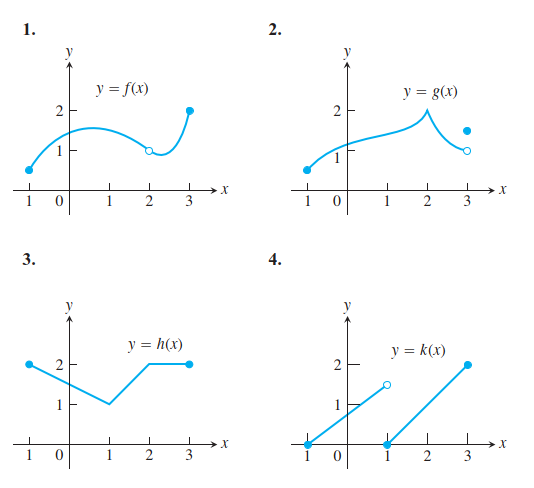
\includegraphics[width=20em]{t13uno}
\end{figure}


\textbf{1.} No es continua en $[-1,3]$, porque no está definida cuando $x=2$

\textbf{2.} No es continua en $[-1,3]$, porque el límite cuando $x \to 3$ es diferente a $g(3)$

\textbf{3.} Si continua en $[-1,3]$, porque está definida para todo punto en ese intervalo.

\textbf{4.} No es continua en $[-1,3]$, porque no existe el límite cuando $x \to 1$


\textbf{En los ejercicios 5 al 10, son acerca de la función}\\

\begin{figure}[tbh]
\centering
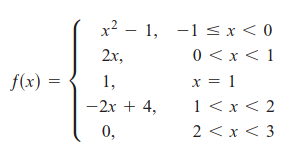
\includegraphics[width=20em]{t13dos}
\end{figure}

cuya gráfica es
\begin{figure}[tbh]
\centering
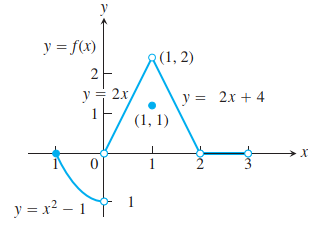
\includegraphics[width=25em]{t13tres}
\end{figure}\\

\textbf{5.a ¿$f(-1)$ existe?} Sí, $f(-1) = 0$\\
\textbf{5.b $\lim_{ x \to -1^+} f(x) $ existe?} Sí, $\lim_{ x \to -1^+} f(x)= 0$\\
\textbf{5.c ¿$\lim_{ x \to -1^+} f(x) = f(-1)$ ?} Sí\\
\textbf{5.d ¿ Es continua $f$ en $x = -1$ ?} Sí\\


\textbf{6.a ¿$f(1)$ existe?} Sí, $f(1) = 1$\\
\textbf{6.b $\lim_{ x \to 1} f(x) $ existe?} Sí, $\lim_{ x \to 1} f(x)= 2$ \\
\textbf{6.c ¿$\lim_{ x \to 1} f(x) = f(1)$ ?} No\\
\textbf{6.d ¿ Es continua $f$ en $x = 1$ ?} No\\


\textbf{7.a ¿Está definida en $x = 2$?} No\\
\textbf{7.b ¿Es $f$ continua en x = 2?} No\\

\textbf{8. ¿En que valores de $x$ es continua $f$?} En los intervalos $(0,1) \cup (1,2) \cup (2,3) \cup \{-1\}$\\


\textbf{9. ¿Qué valor debe asignarse a $f(2)$ para que la función extendida sea continua en $x = 2$?} 0\\


\textbf{10. ¿A qué nuevo valor hay que cambiar $f(1)$ para remover la discontinuidad?} 2\\


\textbf{53.  Una función discontinua en todos los puntos}\\
\textbf{a.} Use el hecho de que todo intervalo no vacío de números reales contiene números racionales e irracionales, para probar que la función
\begin{align*}
f(x)= \left\{ \begin{array}{lcc}
                 1, &   si   & x \text{ es racional} \\
             	\\ 0, &   si   & x \text{ es irracional}
             \end{array}
   \right.
\end{align*}

es discontinua en todos los puntos.

\textbf{b.} $f$ es continua por la derecha o por la izquierda en algún punto? No
 
Una función es continua en un punto si $f(x_0) = \lim_{x \to x_0}$.

Supongo que mi $x_0$ es un número racional, entonces $f(x_0) = 1$, ahora para encontrar el límite me puedo acercar de dos maneras:
Con números racionales con lo que $\lim_{x \to x_0 = 1}$
Y con números irracionales tal que $\lim_{x \to x_0 = 0}$
Como las dos aproximaciones son distintas el $\lim_{x \to x_0}$ no existe.

Ahora supongo que mi $x_0$ es un número irracional, entonces $f(x_0) = 0$, ahora para encontrar el límite me puedo acercar de dos maneras:
Con números racionales con lo que $\lim_{x \to x_0 = 1}$ 
Y con números irracionales tal que $\lim_{x \to x_0 = 0}$
Como las dos aproximaciones son distintas el $\lim_{x \to x_0}$ no existe.

\end{document} 